% Impedanz Ortskurve RLs-Glied
% R=konst. mit R=R0
% wL=var. mit wL=p*w0L0, p in [0,3]
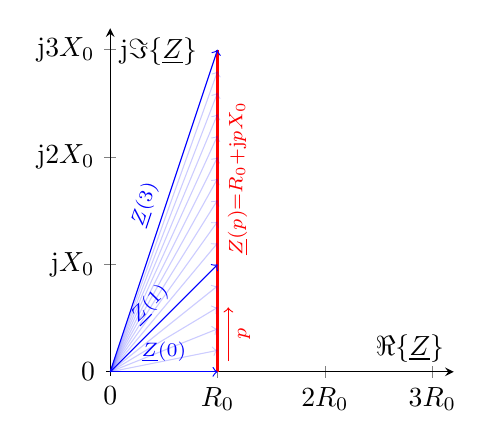
\begin{tikzpicture}
    \begin{axis}[
        xlabel=$\Re\{\underline{Z}\}$,
        ylabel=$\mathrm{j}\Im\{\underline{Z}\}$,
        axis lines=center,
        xmin=-0.2,xmax=16,% scaling: 5/1 = coordinates/shown values
        ymin=-0.2,ymax=16,% scaling: 5/1 = coordinates/shown values
        width=6cm, height=6cm,
        clip=false,
        xtick={0,5,10,15},% tick near center <0.01 not displayed
        xticklabels={,$R_0$,$2R_0$,$3R_0$},
        ytick={0,5,10,15},
        yticklabels={,$\mathrm{j}X_0$,$\mathrm{j}2X_0$,$\mathrm{j}3X_0$},
    ]
        % manual ticks at (0,0)
        \node[anchor=north,yshift=-2pt] at (0,0) {$0$};
        \node[anchor=east,xshift=-2pt] at (0,0) {$0$};
        % Ortskurve
        \addplot[mark=none,thick,red,domain=0:15] ({5},{x})
            node[pos=0.6,below,sloped]{$\scriptstyle\underline{Z}(p)=R_0 + \mathrm{j}pX_0$};
        % Richtungspfeil
        \addplot[->,red] coordinates{(5.5,0.5)(5.5,3.0)}
            node[midway,below,sloped]{$\scriptstyle p$};
        % Zeiger
        \foreach \i in {0,...,15}{\addplot[->,blue,opacity=0.2] coordinates{(0,0)(5,{\i})};}
        \addplot[->,blue] coordinates{(0,0)(5,0)}   % Zeiger p=0
            node[midway,above,sloped]{$\scriptstyle\underline{Z}(0)$};
        \addplot[->,blue] coordinates{(0,0)(5,5)}   % Zeiger p=5
            node[midway,above,sloped]{$\scriptstyle\underline{Z}(1)$};
        \addplot[->,blue] coordinates{(0,0)(5,15)}  % Zeiger p=15
            node[midway,above,sloped]{$\scriptstyle\underline{Z}(3)$};
    \end{axis}
\end{tikzpicture}